% !TeX root=../journalDeepMedic.tex


%%%%%%%%%%%%%%%%%%%%%%%%%%%%%%%%%%%%%%%%%%%%%%%%%%%%%%%%%%%%%%
%%%%%%%%%%% Validation of the Architecture %%%%%%%%%%%%%%%%%%%
%%%%%%%%%%%%%%%%%%%%%%%%%%%%%%%%%%%%%%%%%%%%%%%%%%%%%%%%%%%%%%

\section{Analysis of Network Architecture}
\label{sec:vaOfNetArch}

In this section we present a series of experiments in order to analyze the impact of each of the main contributions and to justify the choices made in the design of the proposed 11-layers, multi-scale 3D CNN architecture, referred to as the \textit{DeepMedic}. Starting from the CNN baseline as discussed in Sec.~\ref{subsec:theBaseline}, we first explore the benefit of our proposed dense training scheme (cf. Sec.~\ref{subsec:denseTraining}), then investigate the use of deeper models (cf. Sec.~\ref{subsec:buildingADeeperNetwork}) and then evaluate the influence of the multi-scale dual pathway (cf. Sec.~\ref{subsec:multiscaleCnn}). Finally, we compare our method with corresponding 2D variants to assess the benefit of processing 3D context.

\subsection{Experimental Setting}
\label{subsec:experimentSetting}

The following experiments are conducted using the TBI dataset with 61 multi-channel MRIs which is described in more detail later in Sec.~\ref{subsec:evalTbi}. Here, the images are randomly split into a validation and training set, with 15 and 46 images each. The same sets are used in all analyses. To monitor the progress of segmentation accuracy during training, we extract 10k random patches at regular intervals, with equal numbers extracted from each of the validation images. The patches are uniformly sampled from the brain region in order to approximate the true distribution of lesions and healthy tissue. Full segmentation of the validation datasets is performed every five epochs and the mean Dice similarity coefficient (DSC) is determined. Details on the configuration of the networks are provided in \ref{app:detailsConfig}.

\subsection{Effect of Dense Training on Image Segments}
\label{subsec:valDenseTraining}

\begin{figure}[!h]
\centering
\begin{subfigure}[b]{1.0\textwidth}
\centering
	%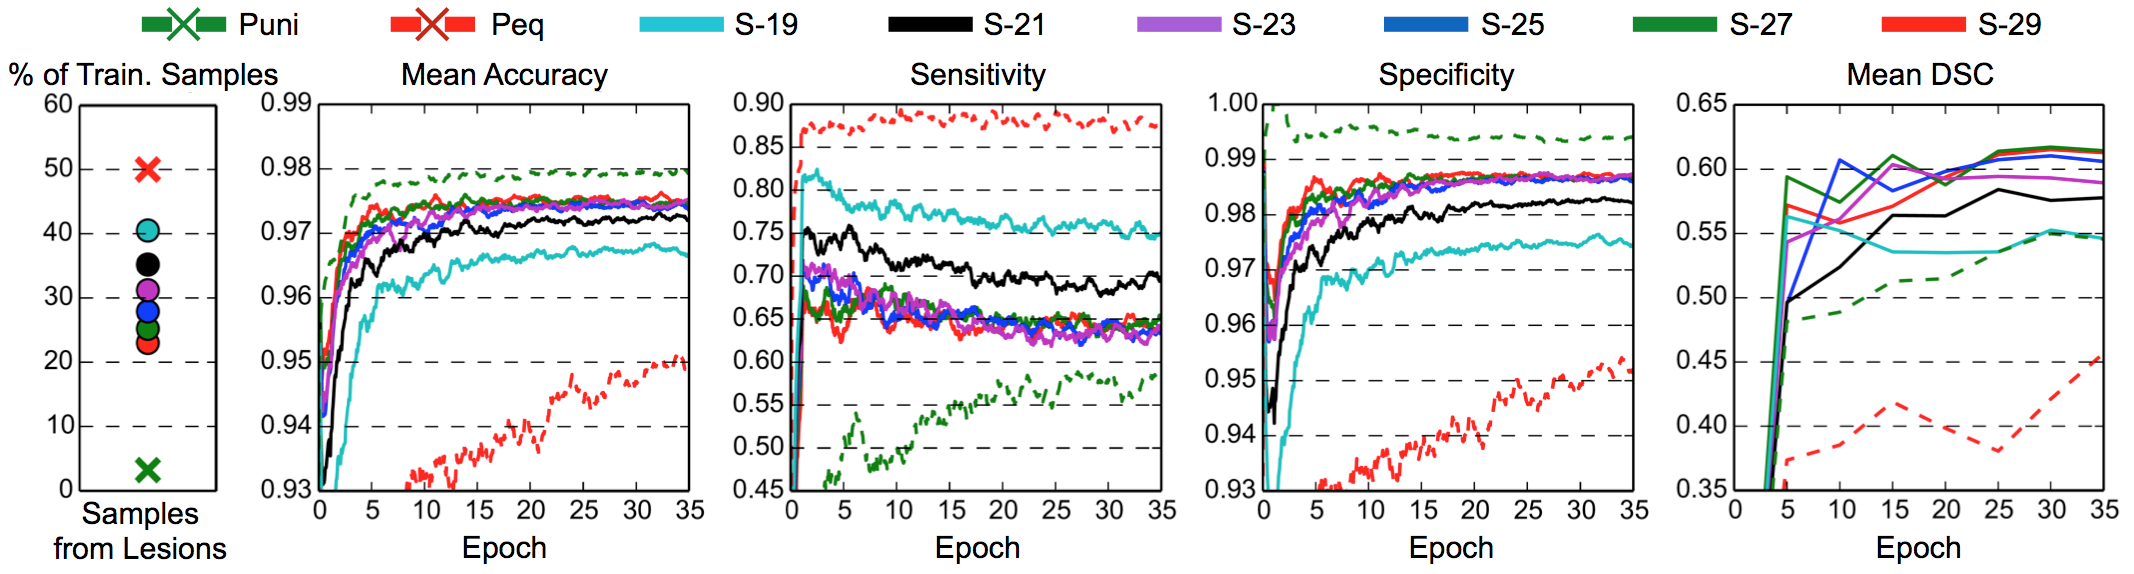
\includegraphics[clip=true, trim=10pt 270pt 30pt 210pt, width=1.0\textwidth]{figures/validationOfArchitecture/denseTraining/denseFigureToPlace.pdf}
	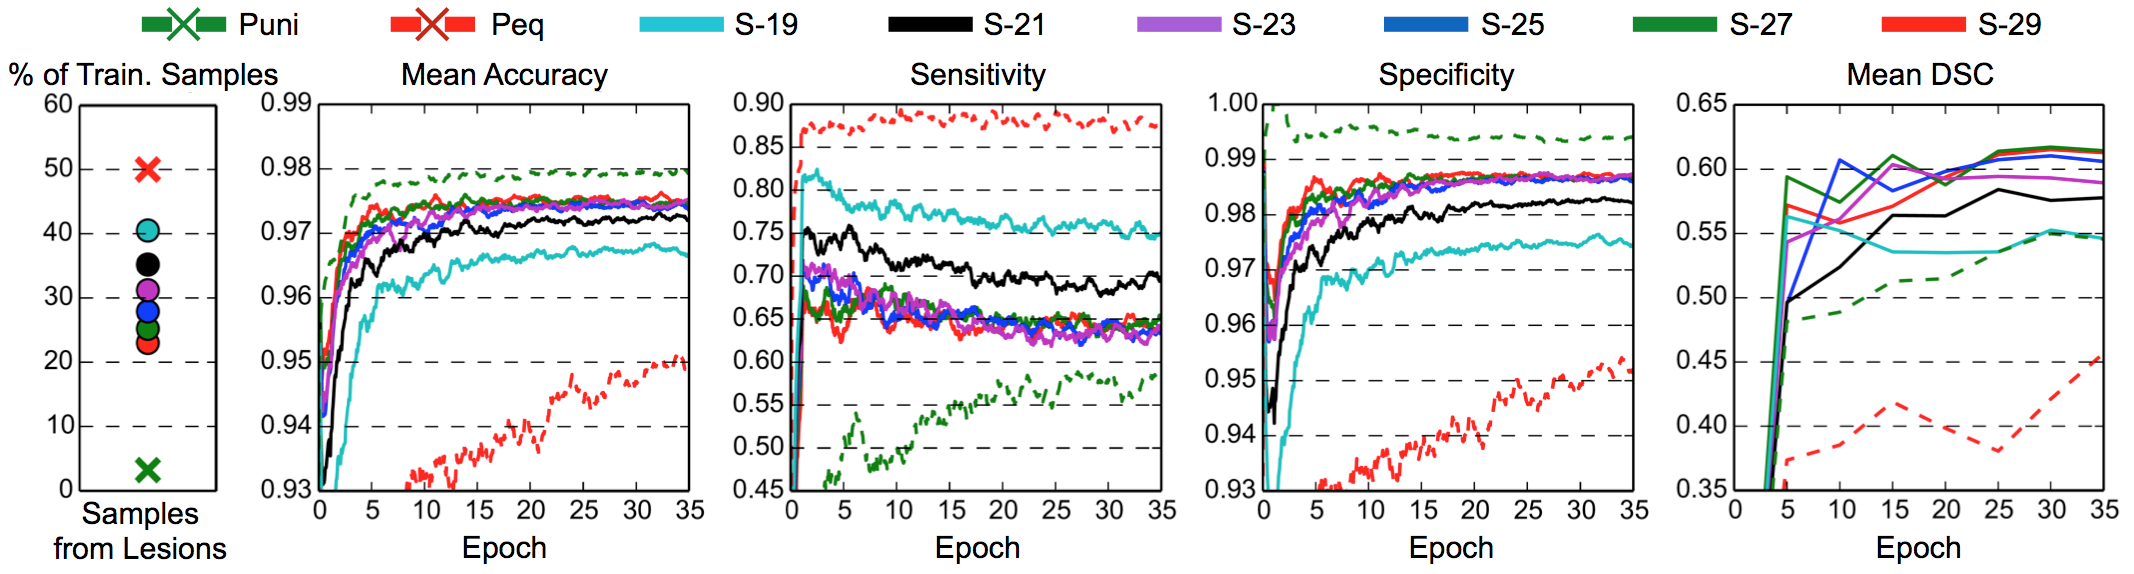
\includegraphics[clip=true, trim=0pt 0pt 0pt 0pt, width=1.0\textwidth]{figures/validationOfArchitecture/denseTraining/denseFigureToPlace.png}
\end{subfigure}
\caption{Comparison of the commonly used methods for training on patches uniformly sampled from the brain region (P$_\text{uni}$) and equally sampled from lesion and background (P$_\text{eq}$) against our proposed scheme (S-${d}$) on cubic segments of side length $d$, also equally sampled from lesion and background. We varied $d$ to observe its effect. From left to right: percentage of training samples extracted from the lesion class, mean accuracy, sensitivity, specificity calculated on uniformly sampled validation patches and, finally, the mean DSC of the segmentation of the validation datasets. The progress throughout training is plotted. Because lesions are small, P$_\text{uni}$ achieves very high voxel-wise accuracy by being very specific but not sensitive, with the opposite being the case for P$_\text{eq}$. Our method achieves an effective balance between the two, resulting in better segmentation as reflected by higher DSC.}
\label{fig:denseTrainingExperiment}
\end{figure}
%\vspace{-1pt} %takes away some white space before figure

We compare our proposed dense training method with two other commonly used training schemes on the 5-layers baseline CNN (see Fig.~\ref{fig:cnnBaseline}). The first common scheme trains on $17^3$ patches extracted uniformly from the brain region, and the second scheme samples patches equally from the lesion and background class. We refer to these schemes as P$_\text{uni}$ and P$_\text{eq}$. The results shown in Fig.~\ref{fig:denseTrainingExperiment} show a correlation of sensitivity and specificity with the percentage of training samples that come from the lesion class. P$_\text{eq}$ performs poorly because of over-segmentation (high sensitivity, low specificity). P$_\text{uni}$ has better classification on the background class (high specificity), which leads to high mean voxel-wise accuracy since the majority corresponds to background, but not particularly high DSC scores due to under-segmentation (low sensitivity).

To evaluate our dense training scheme, we train multiple models with varying sized image segments, equally sampled from lesions and background. The tested sizes of the segments go from $19^3$ upwards to $29^3$. The models are referred to as \quot{S-$d$}, where $d$ is the side length of the cubic segments. For fair comparison, the batch sizes in all the experiments are adjusted to have a similar memory footprint and lead to similar training times as compared to training on P$_{uni}$ and P$_{eq}$\footnote{Dense training on a whole volume was inapplicable in these experimental settings due to memory limitations but was previously shown to give similar results as training on uniformly sampled patches (\cite{Long2014}).}. We observe a great performance increase for model S-${19}$ over P$_\text{eq}$. We account this partly to the efficient increase of the effective batch size ($B \cdot V$ in Eq.~(\ref{eq:costDense})), but also to the altered distribution of training samples. As we increase the size of the training segments further, we quickly reach a balance between the sensitivity of P$_{eq}$ and the specificity of P$_{uni}$, which results in improved segmentation as expressed by the DSC.

The segment size is a hyper-parameter in our model. We observe that the increase in performance with increasing segment size quickly levels off, and similar performance is obtained for a wide range of segment sizes, which allows for easy configuration. For the remaining experiments, all models were trained on segments of size $25^3$.


\subsection{Effect of Deeper Networks}
\label{subsec:valDeeper}

\begin{figure}[!h]
\centering
\begin{subfigure}[b]{0.5\textwidth}
\centering
	%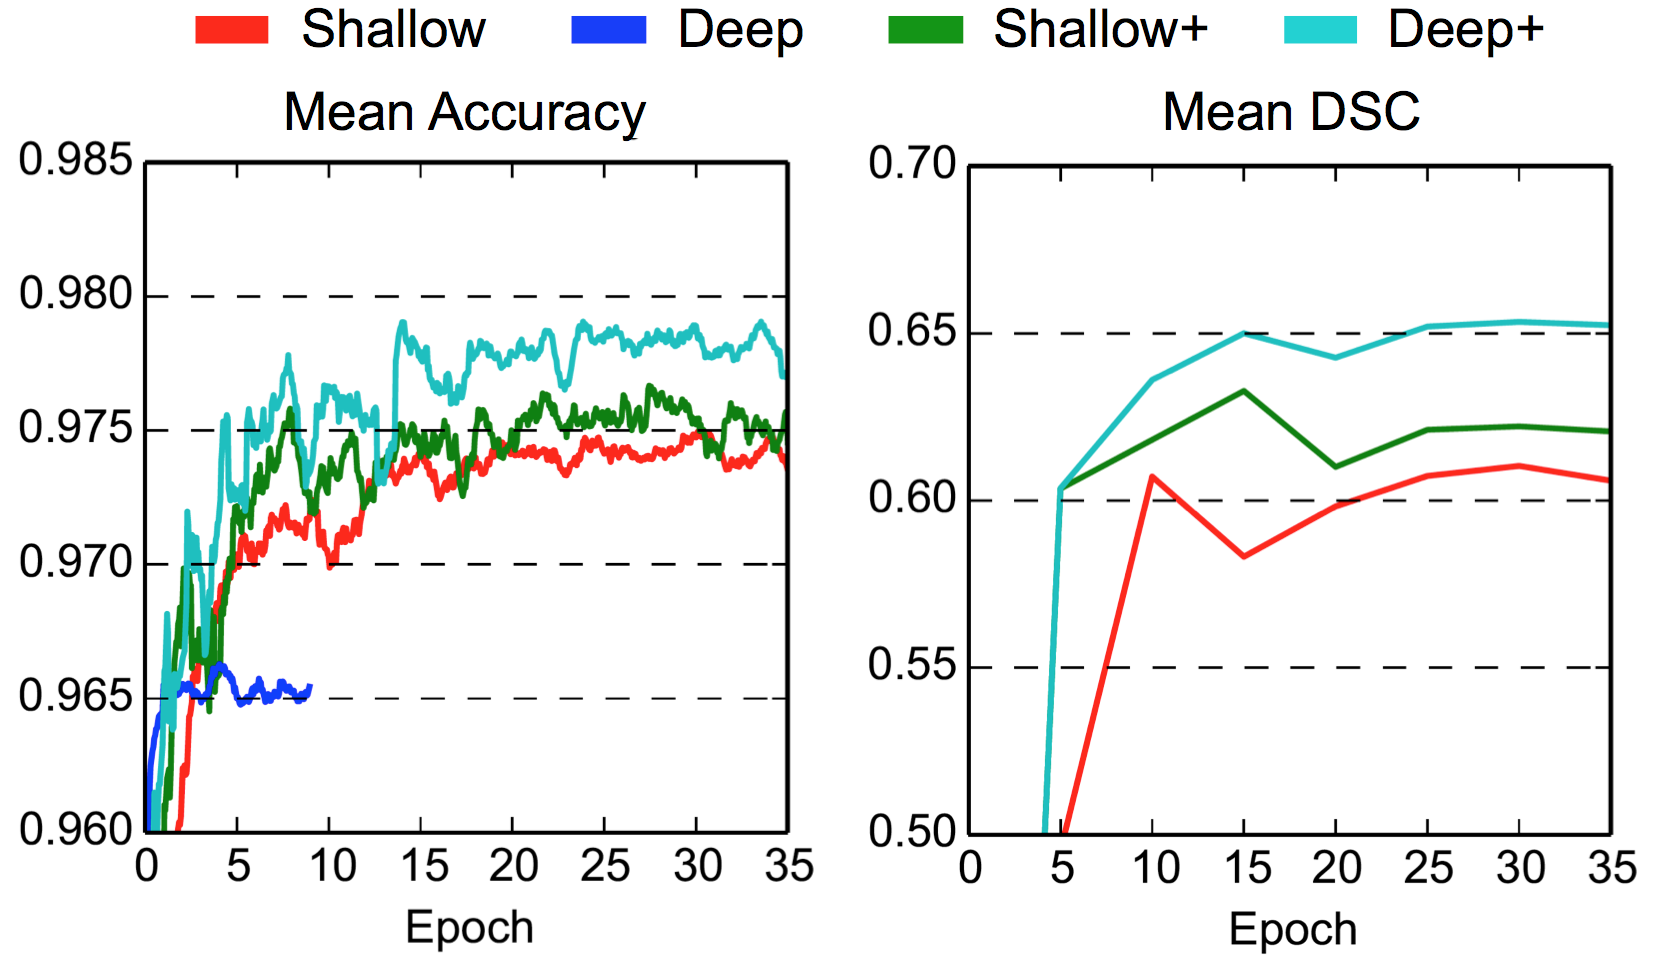
\includegraphics[clip=true, trim=50pt 30pt 140pt 250pt, width=1.0\textwidth]{figures/validationOfArchitecture/deepProblems/deepFigureToPut.pdf}
	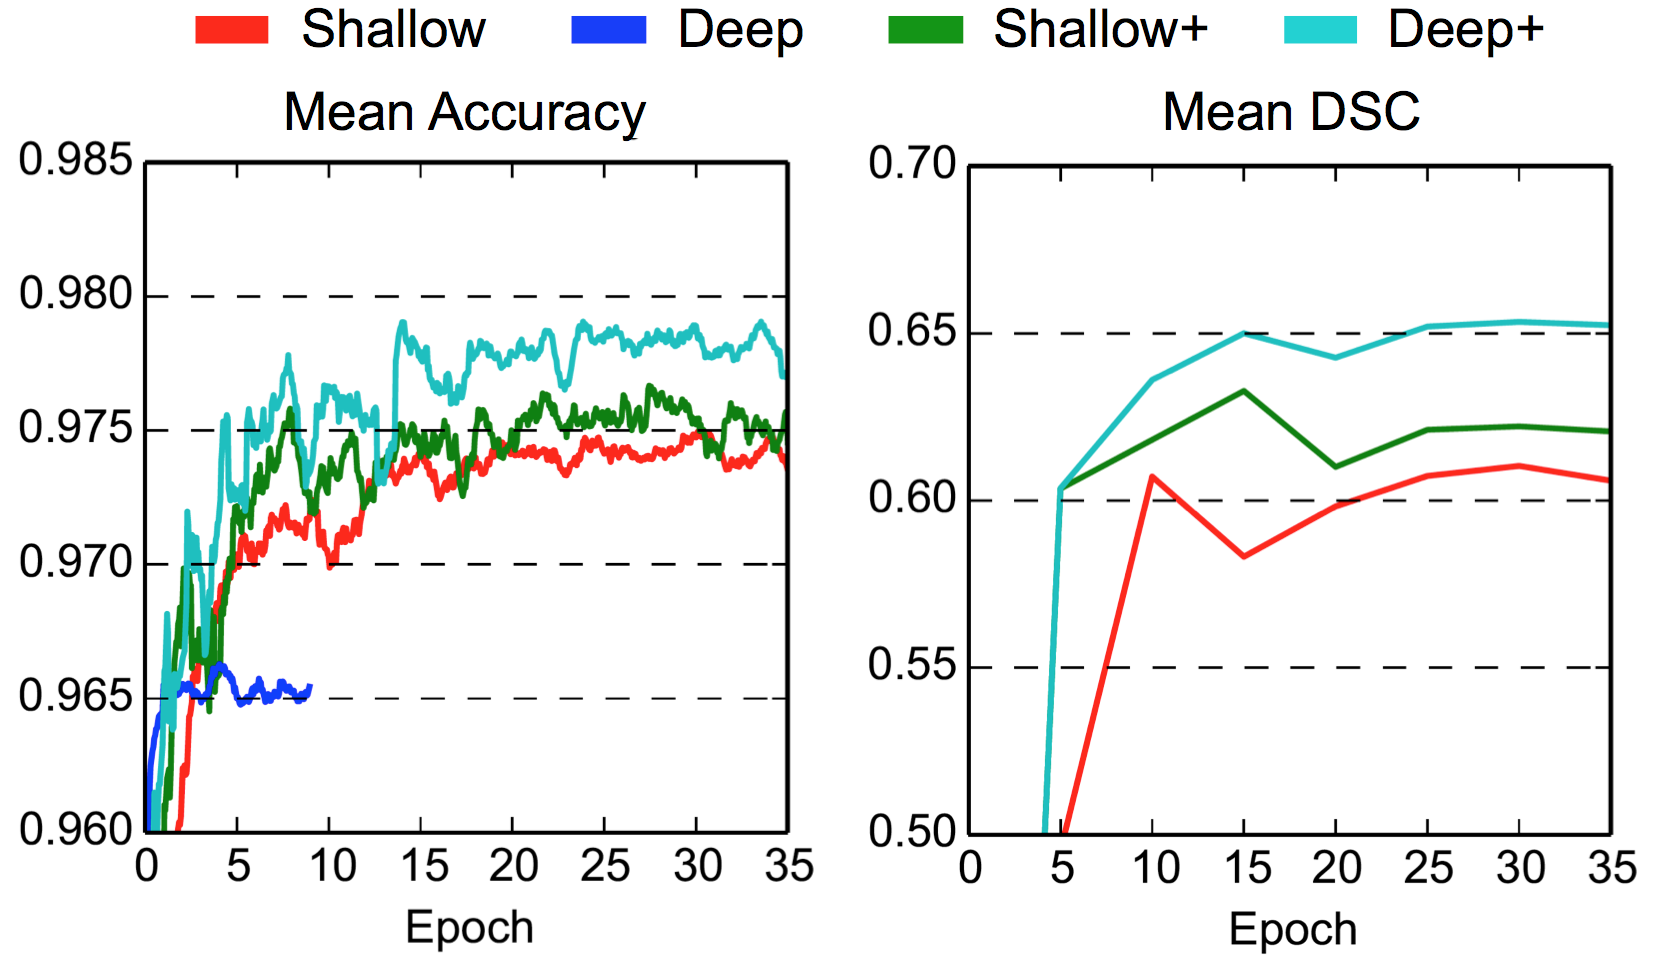
\includegraphics[clip=true, trim=0pt 0pt 0pt 0pt, width=1.0\textwidth]{figures/validationOfArchitecture/deepProblems/deepFigureToPut.png}
\end{subfigure}
\caption{Mean accuracy over validation samples and DSC for the segmentations of the validation images, as obtained from the \quot{Shallow} baseline and \quot{Deep} variant with smaller kernels. Training of the plain deeper model fails (cf. Sec.~\ref{subsec:valDeeper}). This is overcome by adopting the initialization scheme of (\cite{he2015delving}), which further combined with Batch Normalization leads to the enhanced (\texttt{+}) variants. Deep\texttt{+} performs significantly better than Shallow\texttt{+} with similar computation time, thanks to the use of small kernels.
}
\label{fig:deepProblems}
\end{figure}
%\vspace{-1pt} %takes away some white space before figure

The 5-layers baseline CNN (Fig.~\ref{fig:cnnBaseline}), here referred to as the \quot{Shallow} model, is extended to 9-layers by replacing each convolutional layer that uses $5^3$ kernels with two layers that use $3^3$ kernels (Fig.~\ref{fig:deeper3x3}). This model is referred to as \quot{Deep}. Training the latter, however, utterly fails with the model making only predictions corresponding to the background class. This problem is related to the challenge of preserving the signal as it propagates through deep networks and its variance gets multiplied with the variance of the weights, as previously discussed in Sec.~\ref{subsec:buildingADeeperNetwork}. One of the causes is that the weights of both models have been initialized with the commonly used scheme of sampling from the normal distribution $\mathcal{N}(0,0.01)$ (cf. \cite{Krizhevsky2012}). In comparison, the initialization scheme by \cite{he2015delving}, derived for preserving the signal in the initial stage of training, results in higher values and overcomes this problem. Further preservation of the signal is obtained by employing Batch Normalization. This results in an enhanced 9-layers model which we refer to as \quot{Deep\texttt{+}}, and using the same enhancements on the Shallow model yields \quot{Shallow\texttt{+}}. The significant performance improvement of Deep\texttt{+} over Shallow\texttt{+}, as shown in Fig.~\ref{fig:deepProblems}, is the result of the greater representational power of the deeper network. The two models need similar computational times, which highlights the benefits of utilizing small kernels in the design of 3D CNNs. Although the deeper model requires more sequential (layer by layer) computations on the GPU, those are faster due to the smaller kernel size.

\subsection{Effect of the Multi-Scale Dual Pathway}
\label{subsec:valMultiscale}

\begin{figure}[!h]
\centering
\begin{subfigure}[b]{0.5\textwidth}
\centering
	%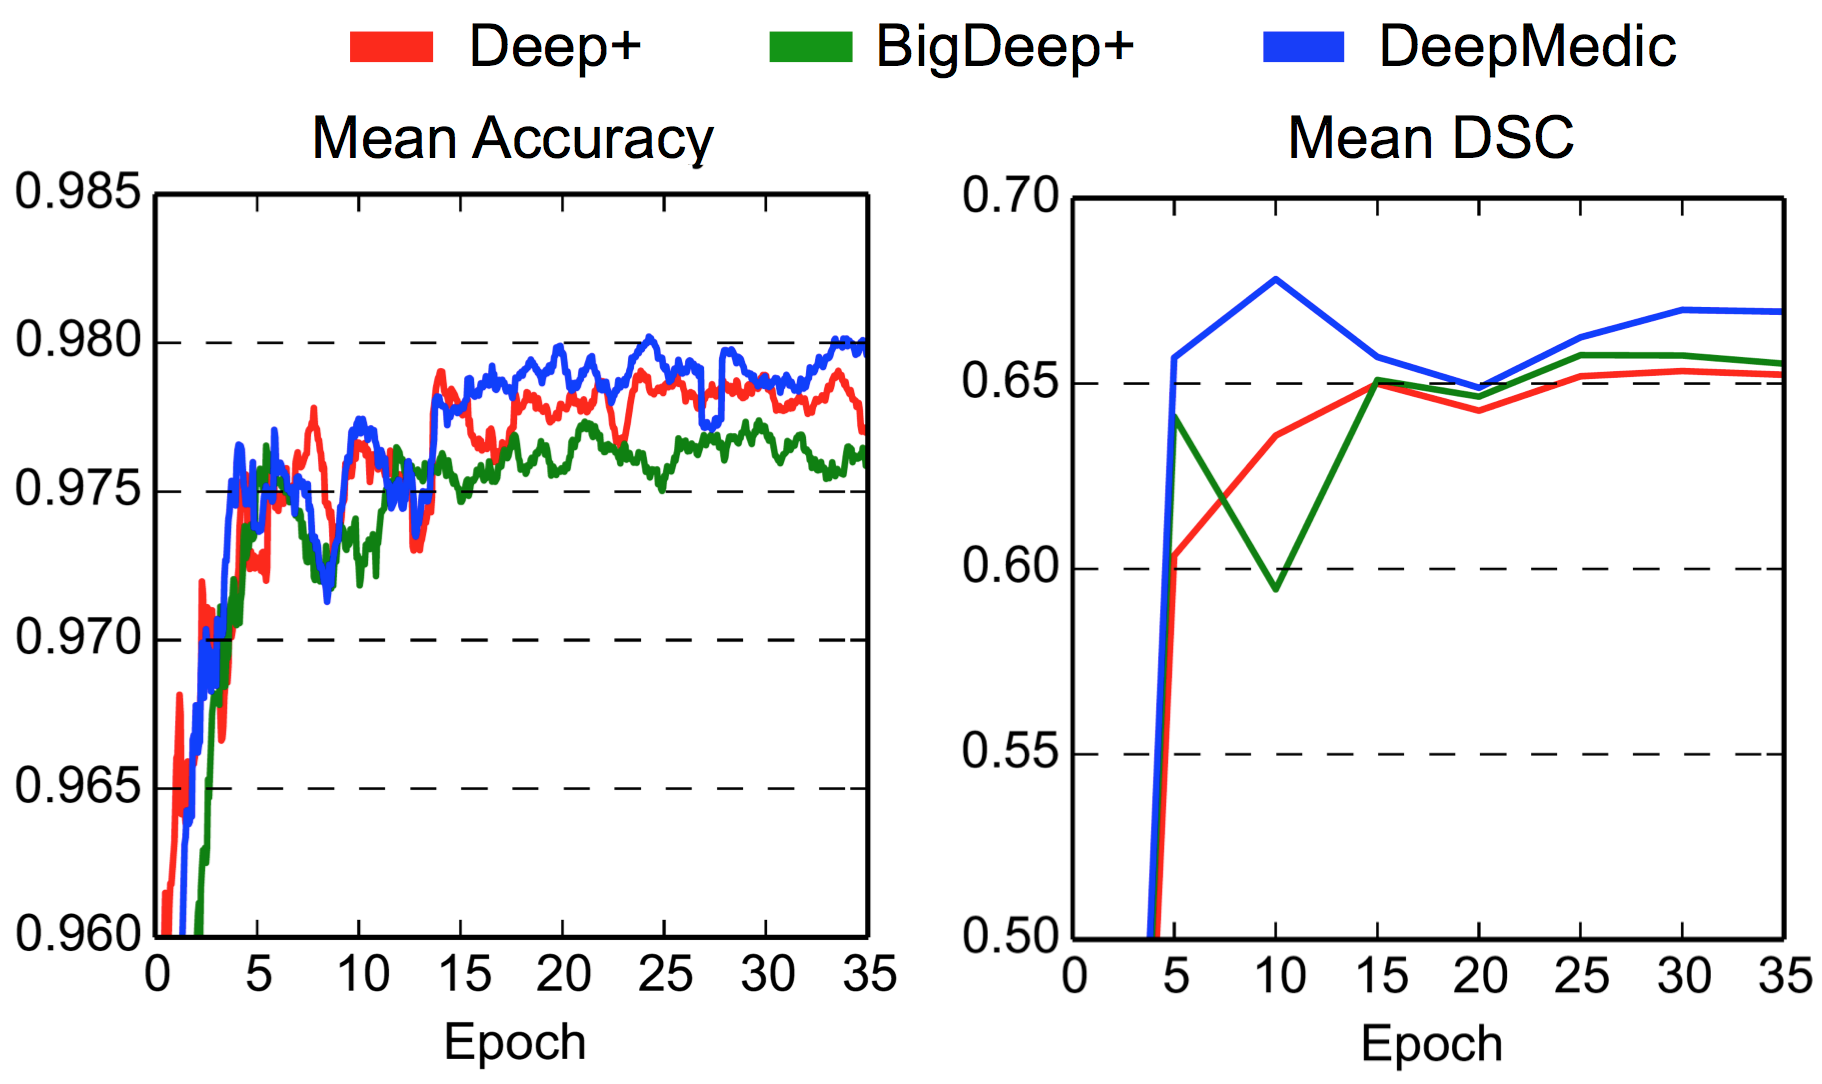
\includegraphics[clip=true, trim=50pt 30pt 140pt 250pt, width=1.0\textwidth]{figures/validationOfArchitecture/multiscale/figureToPut.pdf}
	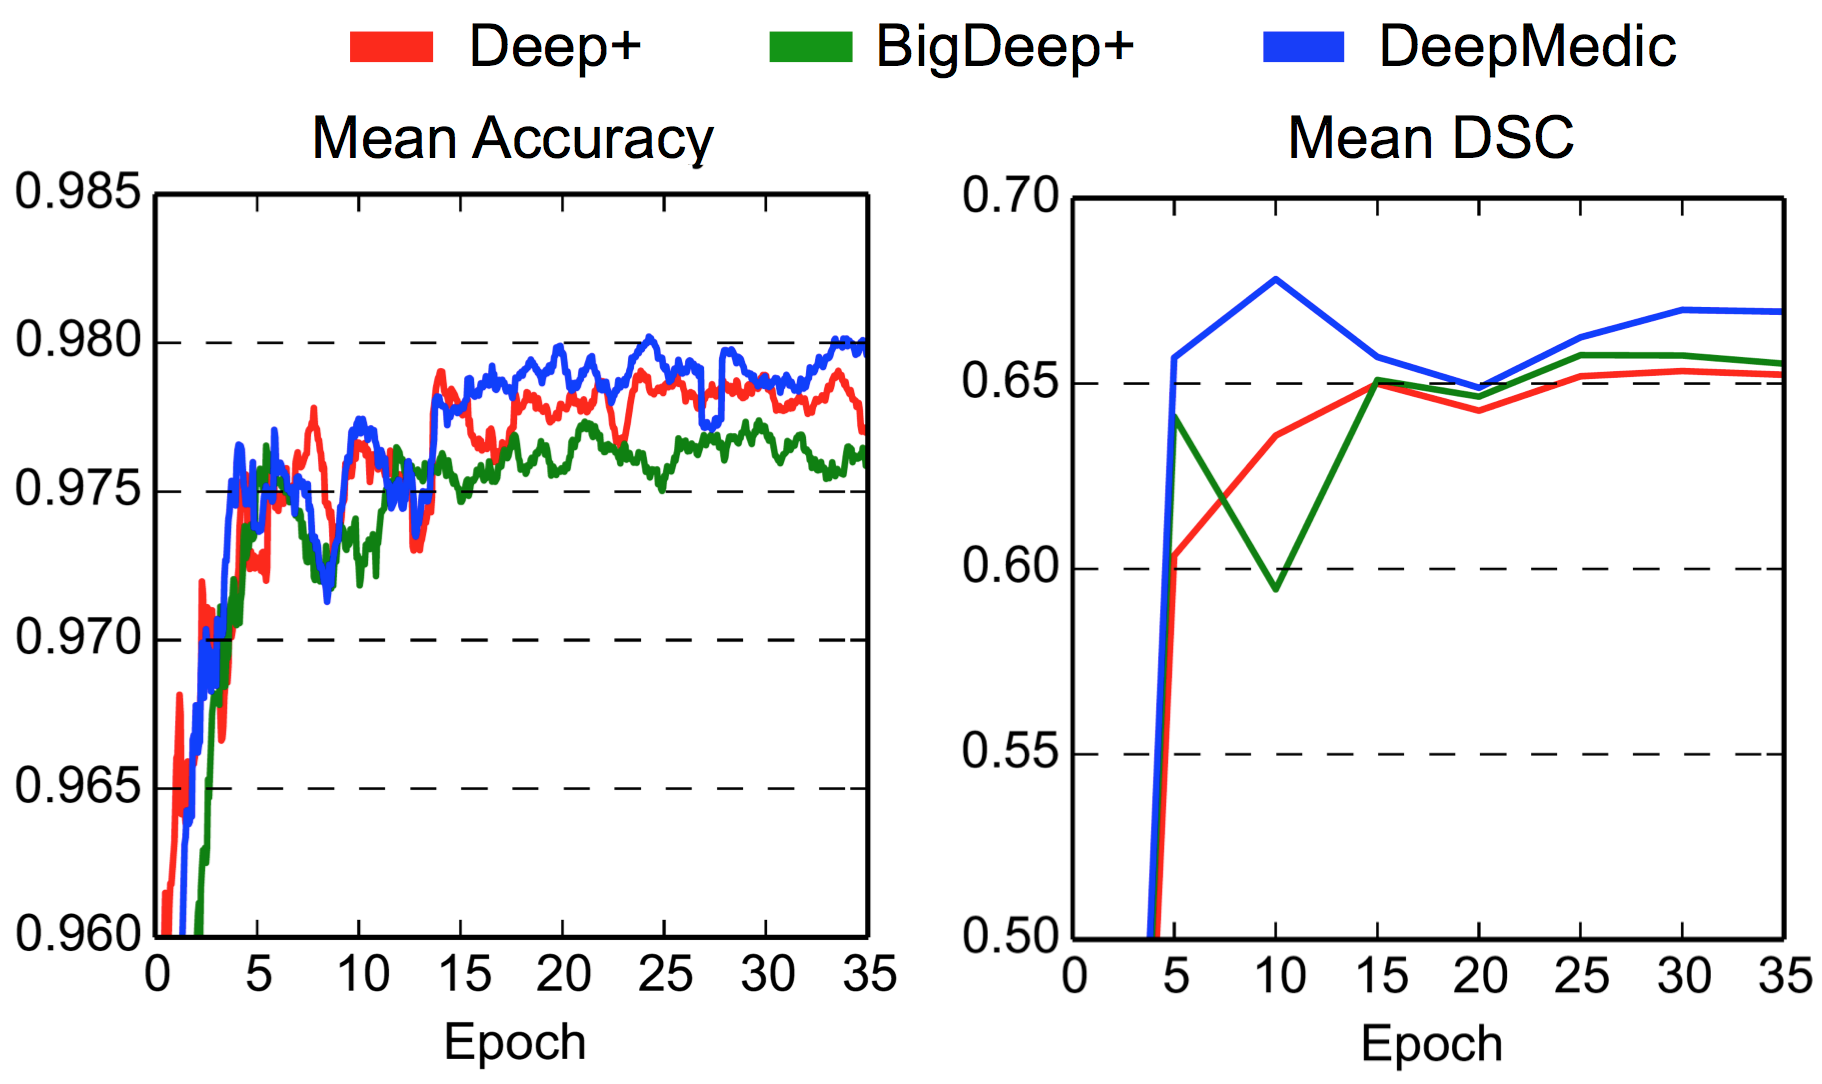
\includegraphics[clip=true, trim=0pt 0pt 0pt 0pt, width=1.0\textwidth]{figures/validationOfArchitecture/multiscale/figureToPut.png}
\end{subfigure}
\caption{Mean accuracy over validation samples and DSC for the segmentation of the validation images, as obtained by a single-scale model (Deep\texttt{+}) and our dual pathway architecture (DeepMedic). We also trained a single-scale model with larger capacity (BigDeep\texttt{+}), similar to the capacity of DeepMedic. DeepMedic yields best performance by capturing greater context, while BigDeep\texttt{+} seems to suffer from over-fitting.
}
\label{fig:multiscaleExperiment}
\end{figure}
%\vspace{-1pt} %takes away some white space before figure

The final version of the proposed network architecture, referred to as \quot{DeepMedic}, is built by extending the Deep\texttt{+} model with a second convolutional pathway that is identical to the first one. Two hidden layers are added for combining the multi-scale features before the classification layer, resulting in a deep network of 11-layers (cf. Fig.~\ref{fig:cnnMultiscale}). The input segments to the second pathway are extracted from the images down-sampled by a factor of three. Thus, the network is capable of capturing context in a $51^3$ area of the original image through the $17^3$ receptive field of the lower-resolution pathway, while only doubling the computational and memory requirements over the single pathway CNN. In comparison, the most recent 2D CNN systems proposed for lesion segmentation (\cite{Havei2015Journal, pereira2015Brats}) have a receptive field limited to $33^2$ voxels.

%+210 to left and -210 to right if I want to move one subfigure.
\begin{figure}[!h]
%\vspace{-1pt} %takes away some white space before figure
\centering
\begin{subfigure}[b]{0.85\textwidth}
\centering
	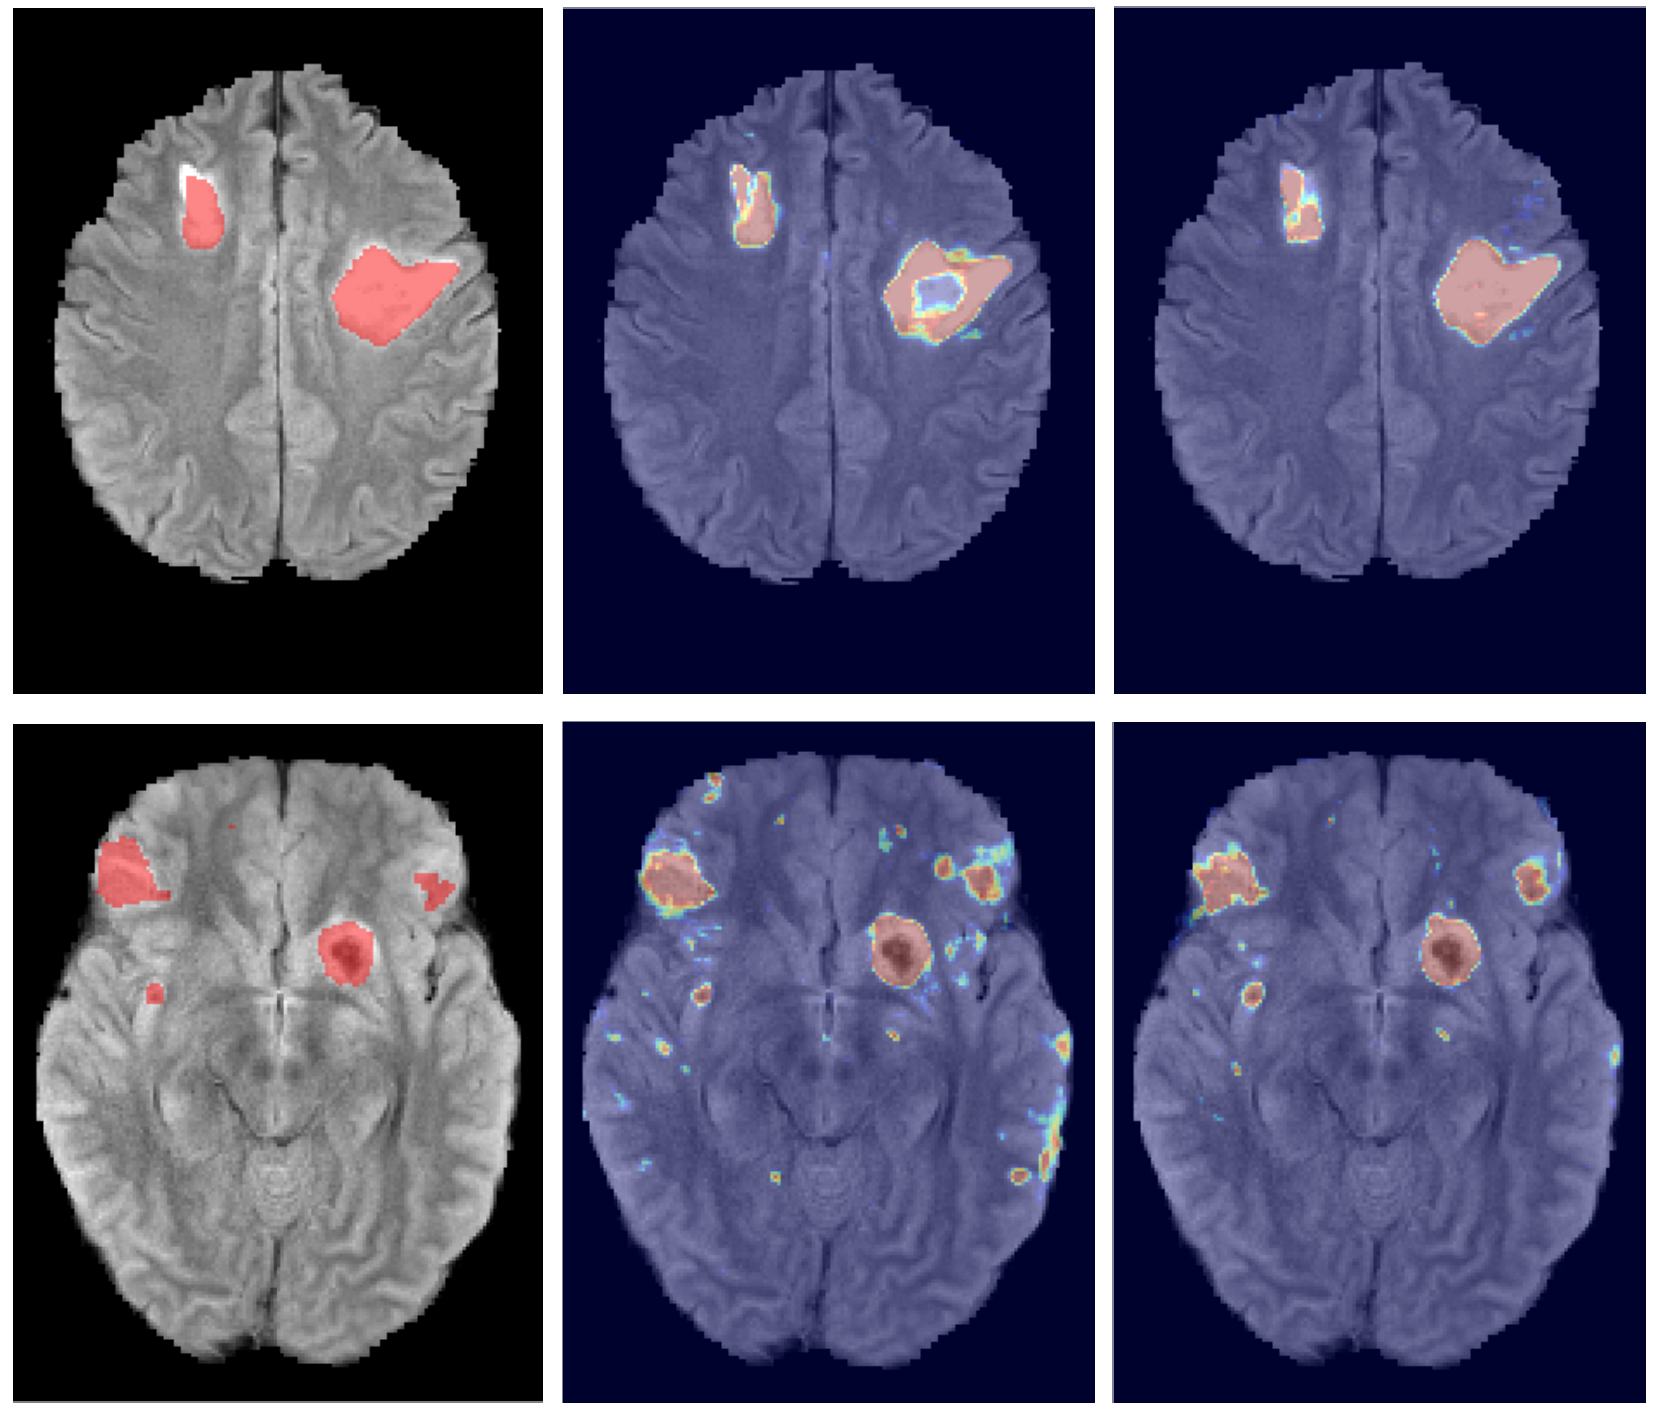
\includegraphics[clip=true, trim=0pt 0pt 0pt 0pt, width=1.0\textwidth]{figures/validationOfArchitecture/multiscale/qualitativeComparisonMultiscale/figureNew/multiscaleQual.png}
\end{subfigure}

\caption{(Rows) Two cases from the severe TBI dataset, showing representative improvements when using the multi-scale CNN approach. (Columns) From left to right: the MRI FLAIR sequence with the manually labeled lesions, predicted soft segmentation map obtained from a single-scale model (Deep\texttt{+}) and the prediction of the multi-scale DeepMedic model. The incorporation of greater context enables DeepMedic to identify when it processes an area within larger lesions (top). Spurious false positives are significantly reduced across the image on the bottom.}
\label{fig:qualitativeMultiscaleVal}
\end{figure}
%\vspace{-1pt} %takes away some white space before figure

Figure~\ref{fig:multiscaleExperiment} shows the improvement DeepMedic achieves over the single pathway model Deep\texttt{+}. In Fig.~\ref{fig:qualitativeMultiscaleVal} we show two representative visual examples of this improvement when using the multi-scale CNN. Finally, we confirm that the performance increase can be accounted to the additional context and not the additional capacity of DeepMedic. To this end, we build a big single-scale model by doubling the FMs at each of the 9-layers of Deep\texttt{+} and adding two hidden layers. This 11-layers deep and wide model, referred to as \quot{BigDeep\texttt{+}}, has the same number of parameters as DeepMedic. The performance of the model is not improved, while showing signs of over-fitting.

\subsection{Processing 3D in comparison to 2D Context}
\label{subsec:val3dContext}

Acquired brain MRI scans are often anisotropic. Such is the case for most sequences in our TBI dataset, which have been acquired with lower axial resolution, except for the isotropic MPRAGE. We perform a series of experiments to investigate the behaviour of 2D networks and assess the benefit of processing 3D context in this setting.

DeepMedic can be converted to 2D by setting the third dimension of each kernel to one. This way only information from the surrounding context on the axial plane influences the classification of each voxel. If 2D segments are given as input, the dimensionality of the feature maps decreases and so does the memory required. This allows developing 2D variants with increased width, depth and size of training batch with similar requirements as the 3D version, which are valid candidates for model selection in practical scenarios. We assess various configurations and present some representatives in Table \ref{subtab:netsConfig2d} along with their performance. Best segmentation among investigated 2D variants is achieved by a 19-layers, multi-scale network, reaching 61.5\% average DSC on the validation fold. The decline from the 66.6\% DSC achieved by the 3D version of DeepMedic indicates the importance of processing 3D context even in settings where most acquired sequences have low resolution along a certain axis.
